\documentclass[11pt]{article}

%\newenvironment{sloppypar*}
% {\sloppy\ignorespaces}
% {\par}


\usepackage[T1]{fontenc}
\usepackage[utf8]{inputenc}
\usepackage{lmodern}
\usepackage{url}
\usepackage[english]{babel}
\usepackage{hyperref}
\usepackage{csquotes}
\usepackage[margin=1in]{geometry}
\usepackage{graphicx} 

\setlength{\parindent}{0em}
\setlength{\parskip}{1em}

\begin{document}

\textbf{Assignment 1 - Applied Econometrics - ECON6645}

\textbf{2022-01-25}

\textbf{Justin Desrosier}

\noindent\rule{16.51cm}{0.4pt}

\textbf{Question 1}

1a)

{
\begin{table}[ht]
\caption{birth weight on GDP per capita}
\centering
\def\sym#1{\ifmmode^{#1}\else\(^{#1}\)\fi}
\begin{tabular}{l*{1}{c}}
\hline\hline
            &\multicolumn{1}{c}{(1)}\\
            &\multicolumn{1}{c}{birth\_weight}\\
\hline
gdp\_cap     &      0.0333\sym{***}\\
            &     (16.97)         \\
[1em]
\_cons      &      2036.5\sym{***}\\
            &     (22.60)         \\
\hline
\(N\)       &         100         \\
\hline\hline
\multicolumn{2}{l}{\footnotesize \textit{t} statistics in parentheses}\\
\multicolumn{2}{l}{\footnotesize \sym{*} \(p<0.05\), \sym{**} \(p<0.01\), \sym{***} \(p<0.001\)}\\
\end{tabular}
\end{table}
}

Table 1 presents the relationship between birth weight and GDP per capita. The coefficient in table 1 for the simple linear regression of birth weight on GDP per capita indicates that a 1 US dollar increase in GDP per capita is on average associated with an increase in birth weights by 0.033 grams. The result is statistically significant at the 1\% level. There is also reason to believe that the independent variable, GDP per capita, is correlated with the error term. Since birth weight is an indication of health levels, healthier workers may lead to a more productive economy and have children healthier children. Therefore, life expectancy may be an omitted variable.  

1b)

\begin{figure}[htbp]
\caption{}\label{fig1}
\begin{center}
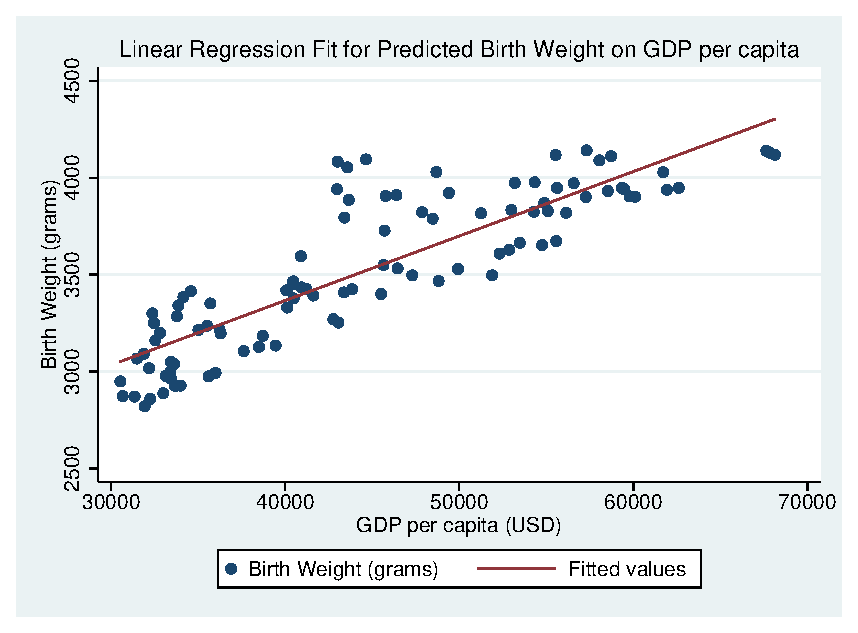
\includegraphics[height=3in]{graph1.eps}
\end{center}
\end{figure}

\textbf{Question 2}

{
\begin{table}[ht]
\caption{health effects}
\centering
\def\sym#1{\ifmmode^{#1}\else\(^{#1}\)\fi}
\begin{tabular}{l*{3}{c}}
\hline\hline
            &\multicolumn{1}{c}{(1)}&\multicolumn{1}{c}{(2)}&\multicolumn{1}{c}{(3)}\\
            &\multicolumn{1}{c}{health}&\multicolumn{1}{c}{health}&\multicolumn{1}{c}{health}\\
\hline
ln\_income   &      0.0690\sym{***}&      0.0693\sym{***}&      0.0732\sym{***}\\
            &     (39.56)         &     (39.66)         &     (41.04)         \\
[1em]
educ\_yrs    &     0.00440\sym{***}&     0.00443\sym{***}&     0.00398\sym{***}\\
            &     (12.73)         &     (12.81)         &     (11.34)         \\
[1em]
age         &    -0.00184\sym{***}&    -0.00423\sym{***}&    -0.00460\sym{***}\\
            &    (-18.60)         &     (-4.68)         &     (-5.03)         \\
[1em]
$age^{2}$ &                     &   0.0000264\sym{**} &   0.0000316\sym{**} \\
            &                     &      (2.67)         &      (3.17)         \\
[1em]
imm         &                     &                     &      0.0580\sym{***}\\
            &                     &                     &      (6.61)         \\
[1em]
ysm         &                     &                     &   -0.000914\sym{**} \\
            &                     &                     &     (-2.60)         \\
[1em]
imm\_ysm123  &                     &                     &     0.00730         \\
            &                     &                     &      (0.46)         \\
[1em]
\_cons      &       0.111\sym{***}&       0.158\sym{***}&       0.121\sym{***}\\
            &      (5.67)         &      (6.00)         &      (4.53)         \\
\hline
\(N\)       &       30371         &       30371         &       29444         \\
\hline\hline
\multicolumn{4}{l}{\footnotesize \textit{t} statistics in parentheses}\\
\multicolumn{4}{l}{\footnotesize \sym{*} \(p<0.05\), \sym{**} \(p<0.01\), \sym{***} \(p<0.001\)}\\
\end{tabular}
\end{table}
}

2a)

Table 2(1) presents the relationship between health as a function of income, education, and age. The coefficients in table 2 for the multiple linear regression indicate that a 1 percent increase in income is associated with a 0.069 unit increase in the health index, an increase in education by 1 year is expected to increase the health index by 0.004 units, and a 1 year increase in age is expected to reduce the health index by 0.002 units. There is likely omitted variable bias in our regression results due to excluding other determinants of health besides age such as exercise, diet, and genetics. Each coefficient is statistically significant at the 1\% level so we can reject the null hypothesis that there is no statistical relationship between the explanatory variables, income, education, and age, and the response variable, health.

2b)

Table 2(2) presents the relationship between health as a function of income, education, age, and $age^{2}$. Adding the quadratic term $age^{2}$ to the model indicates that the effect of age changes when the observations (people) get older. When age is 0, the slope of the fitted regression line is such that the health index would decrease by 0.004 for an increase in age by 1 year if the slope remains unchanged. However, since the $age^{2}$ term has a statistically significant p-value, this would indicate that the slope does not remain unchanged as age increases. The coefficient for $age^{2}$ would indicate that there is an expected increase in the slope by 0.002 units of the health index for 1 additional year of age. Since the coefficient is positive, the relationship between health and age is convex \footnote[1]{https://stats.stackexchange.com/questions/211534/how-to-interpret-quadratic-terms}.

2c)

Table 2(3) presents the relationship between health as a function of income, education, age, $age^{2}$, an immigration dummy variable, and years since migration which equals 0 for Canadian-born respondents and counts the number of years since arrival for immigrants. In particular, Table 2(3) can be used to investigate the "Healthy Immigrant Effect" that posits a tendency for immigrants' health levels to be higher than the Canadian average upon arrival and converge over the years since migration. To test this there is an immigrant dummy variable interacted with a years since migration value of 1, 2, or 3. The coefficient for this variable indicates the expected level of the health index for an immigrant within the first 3 years of arrival in comparison to the average health level of the whole sample. The coefficient for this variable indicates that being an immigrant within the first 3 years of arrival is associated with an expected health index 0.007 units above the average while controlling for income, age, and years of education. We can also see the "Healthy Immigrant Effect" by looking at the years since migration variable. The coefficient for YSM indicates that the slope of the relationship between the health index and years since migration is declining by 0.09 units for each additional year since migration while controlling for the other explanatory variables.

\textbf{Question 3}

3a)

{
\begin{table}[!ht]
\caption{education level and region of residence weightings, effects on wage}
\centering
\def\sym#1{\ifmmode^{#1}\else\(^{#1}\)\fi}
\begin{tabular}{l*{2}{c}}
\hline\hline
            &\multicolumn{1}{c}{(1)}&\multicolumn{1}{c}{(2)}\\
            &\multicolumn{1}{c}{wage}&\multicolumn{1}{c}{wage}\\
\hline
experience  &       0.312\sym{***}&       0.338\sym{***}\\
            &     (18.06)         &     (19.27)         \\
[1em]
union       &       2.259\sym{***}&       1.953\sym{***}\\
            &      (5.90)         &      (5.12)         \\
[1em]
manager     &       8.860\sym{***}&       8.673\sym{***}\\
            &     (18.07)         &     (18.16)         \\
[1em]
big\_firm    &       5.799\sym{***}&       5.734\sym{***}\\
            &     (10.13)         &     (10.39)         \\
[1em]
1.educ\_level.Less Than HS&      -14.21\sym{***}&      -14.62\sym{***}\\
            &    (-19.25)         &    (-22.83)         \\
[1em]
2.educ\_level.HS&      -12.23\sym{***}&      -12.94\sym{***}\\
            &    (-16.60)         &    (-20.72)         \\
[1em]
3.educ\_level.College&      -8.201\sym{***}&      -8.483\sym{***}\\
            &    (-13.94)         &    (-16.89)         \\
[1em]
5.educ\_level.Masters or Higher&       5.619\sym{***}&       5.163\sym{***}\\
            &      (4.98)         &      (5.65)         \\
[1em]
Region.Atlantic Canada    &      -3.809\sym{***}&      -3.803\sym{***}\\
            &     (-8.42)         &     (-7.22)         \\
[1em]
Region.Quebec    &      -3.387\sym{***}&      -3.435\sym{***}\\
            &     (-8.70)         &     (-7.86)         \\
[1em]
Region.Prairies    &       2.403\sym{***}&       2.604\sym{***}\\
            &      (4.83)         &      (4.46)         \\
[1em]
Region.British Columbia    &       0.381         &     -0.0831         \\
            &      (0.56)         &     (-0.10)         \\
[1em]
\_cons      &       26.91\sym{***}&       26.89\sym{***}\\
            &     (41.27)         &     (43.18)         \\
\hline
\(N\)       &       11406         &       11406         \\
\hline\hline
\multicolumn{3}{l}{\footnotesize \textit{t} statistics in parentheses}\\
\multicolumn{3}{l}{\footnotesize \sym{*} \(p<0.05\), \sym{**} \(p<0.01\), \sym{***} \(p<0.001\)}\\
\end{tabular}
\end{table}
}

Table 3(1) and 3(2) present the results from a multiple linear regression of wage on experience, union membership, having a managerial position, and working for a large firm, while also controlling for specific education level effects and specific region of residence effects. For the education level and region of residence specific effects, Bachelor's Degree and Ontario are the reference categories. Model (1) has a probability weighting for region of residence strata and model (2) has a probability weighting for education level strata. Population weights for the education level strata in (2) is the more robust model since the standard errors are lower or the same for all explanatory variables with the exception of the British Columbia regional dummy variable. 

The results from model (2) indicate that a 1 year increase in experience is associated with a 0.34 cent increase in hourly wages, membership in a union is associated with 1.95 dollar increase in hourly wages, being a manager is associated with an 8.67 dollar increase in hourly wages, and being employed in a firm with 1000 or more employees is associated with a 5.73 dollar increase in hourly wages. 

In terms of the educational attainment categorical variable, where a Bachelor's Degree is the reference level of education, the sample average hourly wage for someone with: Less Than HS is 14.62, HS 12.94, and College 8.48 dollars less than the average hourly wage for someone with a Bachelor's Degree. Sample average hourly wage is 5.16 dollars higher for someone with Masters or Higher education level compared to the average hourly wage for someone with a Bachelor's Degree.

For the region of residence categorical variable with Ontario as the reference region, the coefficients indicate that working in Atlantic Canada is associated with an average hourly wage 3.80 dollars less than the average hourly wage in Ontario. For workers in Quebec and British Columbia, their average wages are expected to be 3.43 and 0.08 dollars less than the average wage in Ontario respectively. In the Prairies, the average worker can expected to have wages 2.60 dollars higher than the average hourly wage in Ontario. 

3b)

{
\begin{table}[!ht]
\caption{effects on wage for females}
\centering
\def\sym#1{\ifmmode^{#1}\else\(^{#1}\)\fi}
\begin{tabular}{l*{1}{c}}
\hline\hline
            &\multicolumn{1}{c}{(1)}\\
            &\multicolumn{1}{c}{wage}\\
\hline
educ\_yrs    &       2.075\sym{***}\\
            &     (21.57)         \\
[1em]
1.female    &      -3.413         \\
            &     (-1.55)         \\
[1em]
$1.female\times c.educ\_yrs$&     0.00997         \\
            &      (0.07)         \\
[1em]
experience  &       0.340\sym{***}\\
            &     (14.43)         \\
[1em]
$1.female\times c.experience$&   -0.117\sym{***}\\
            & (-3.42)         \\
[1em]
1.union     &  0.898         \\
            &  (1.62)         \\
[1em]
$1.union\times 1.female$&  2.427\sym{**} \\
            &   (3.11)         \\
[1em]
1.manager   &   11.54\sym{***}\\
            &   (19.24)         \\
[1em]
$1.manager\times 1.female$&   -5.126\sym{***}\\
            &        (-5.83)         \\
[1em]
1.big\_firm  &  7.012\sym{***}\\
            &    (9.71)         \\
[1em]
$1.big\_firm\times 1.female$&     -2.814\sym{**} \\
            &     (-2.78)         \\
[1em]
\_cons      &      -7.150\sym{***}\\
            &     (-4.68)         \\
\hline
\(N\)       &       11509         \\
\hline\hline
\multicolumn{2}{l}{\footnotesize \textit{t} statistics in parentheses}\\
\multicolumn{2}{l}{\footnotesize \sym{*} \(p<0.05\), \sym{**} \(p<0.01\), \sym{***} \(p<0.001\)}\\
\end{tabular}
\end{table}
}

Table 4(1) present the results from a multiple linear regression of wage on experience, union membership, having a managerial position, and working for a large firm, as well as the same variables interacted with being female. From model (1) we can see that being female is associated with expected average hourly wages that are 3.41 dollars less than the sample average hourly wage. 

Returns to education for females is expected to be associated with higher average hourly wages, 1 more year of education for females is associated with an increase in hourly wages of 2.09 dollars. Slightly greater than the sample average increase in the hourly wages for an associated 1 year increase in years educated at 2.08 dollars.

Females with 1 additional year of experience on the other hand can expect 0.11 cents less of an increase in their average hourly wage compared to the sample average increase of 0.34 cents. 1 additional year of experience is associated with an increase of hourly wages by 0.23 cents for females. For the average worker, being in a union is expected to result in hourly wages that are 0.90 cents higher than the sample. However, being female and in a union is associated with a 3.33 dollar increase in hourly wages. 

Female managers are expected to make 5.13 dollars less than the average manager, but this is still 6.41 dollars higher than the sample average hourly wage. Similarly, being a female worker in a big firm is associated with a 2.81 dollars less hourly wages than the average worker in a big firm, however this is still 4.20 dollars higher than the sample average hourly wage.

\end{document}